\section{Work Done}
  In this next section I will discuss the work that was carried on the project. In our team we have \textit{'ways of working'}
  flowchart that helps guides us in how the project should be done throughout the team (GoRetro, 2023). Our ways of working is broken down into 5 sections, 
  all of which will be discussed. For a full diagram of our workflow see \hyperref[sec:AppendixD]{\textbf{Appendix D}}.

  \subsection{Requirements and epic creation}
  The First stage is initiation, what's the project going to be about, how it fits into the companies strategy and OKRs, requirement gathering 
  and epic creation, an epic being a set of user stories/features (Karolis, Saulius, 2023).

  \begin{figure}[H]
    \centering
    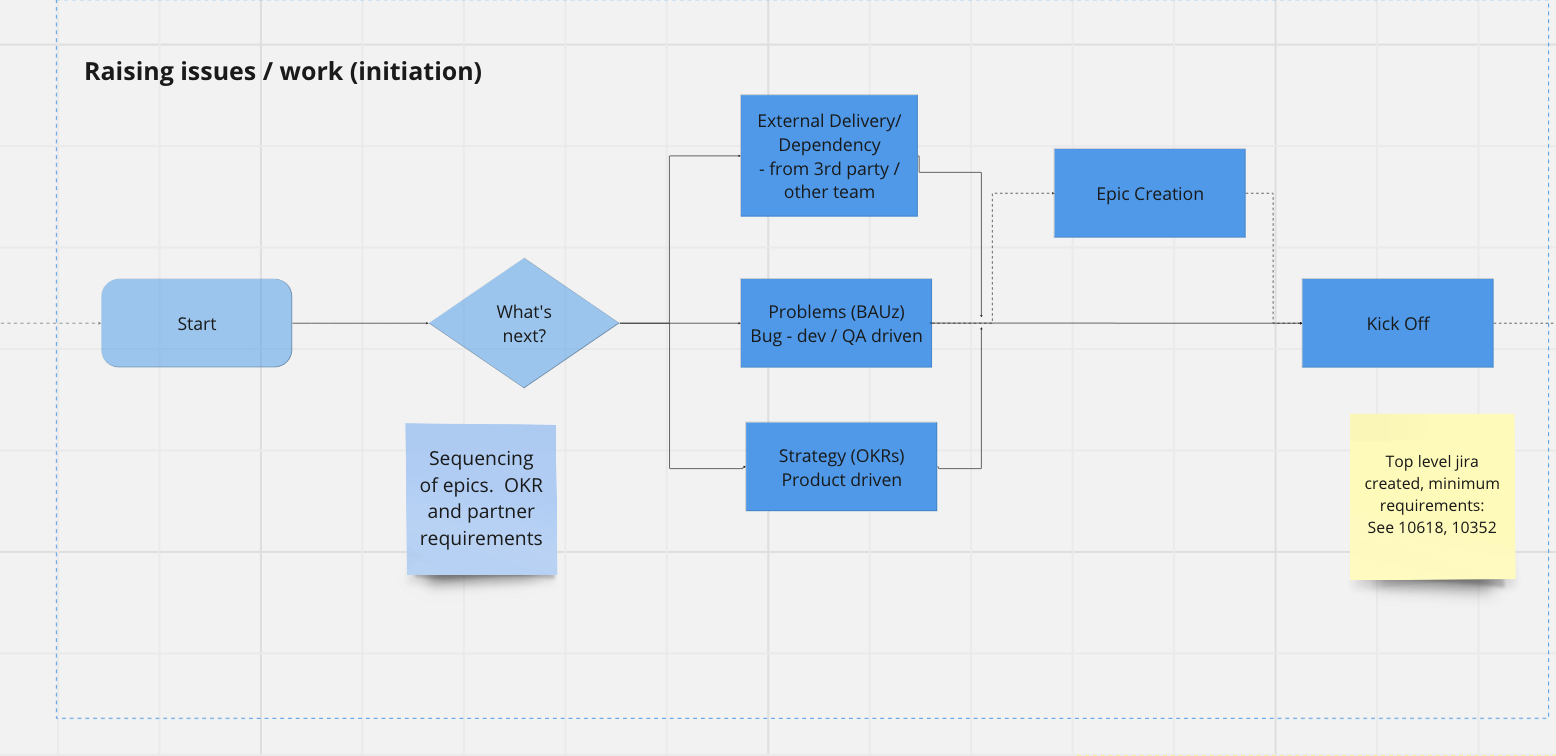
\includegraphics[width=8cm]{assets/workflow/initiate.png}
    \caption{Initiation stage of our ways of working.}
    \label{fig:workflowInitiate}
  \end{figure}

  Due to complications in project allocation, I was not involved in the initial phases of development for this project. However discussions with 
  people that were, highlighted that due to the lack of external partner interaction their wasn't much to discuss and no solid requirements were 
  outlined, only the goal which is to allow the schedule generator to be moved from a static refresh of schedules to an event driven process.

  The benefits of the project and how it achieves our OKRs has been discussed previously in the report. However I want to create some tangible
  requirements here using the MoSCoW framework which consists of must, should, could and won't haves (Eduardo, 2022). I will focus on software
  requirements and denote whether they are functional (F) or non-functional (NF) (Bigelow 2020).

  \begin{enumerate}
    \item (F) The software \textbf{Must} be able to process schedule updates. 
    \item (F) The software \textbf{Must} be able to process episode updates.
    \item (F) The software \textbf{Must} be able to process ancestor updates.
    \item (NF) The software \textbf{Must} keep stored data more relevant than the static version.
    \item (F) The software \textbf{Must} still support a coldstart option.
    \item (F) The software \textbf{Must} contain alarms to alert us to errors.
    \item (F) The software \textbf{Should} gather metrics on processing time and types of updates.
    \item (F) The software \textbf{Should} clean up unneeded data from it's store.
    \item (NF) The software \textbf{Could} support parallelised processing.
  \end{enumerate}

  In this case requirement gathering was easy as there were no partners to discuss the changes with as it's all internal and the output to partners
  stays the same. If this wasn't the case then requirements would have to be gathered from all partners affected or interested in the projects 
  outcome. These requirements would be gathered through meetings and conversations with these partners individually and compromises may have to 
  be made by both sides.
  This is usually the case when there is a requirement conflict, which can be described as:
  \begin{quote}
    \textit{'Requirements conflict is defined as unexpected or contradictory interaction between requirements that has a negative 
    effect on the results (Cameron, Velthuijsen, cited in Kim et al, 2007)'}
  \end{quote}
  These conflicts need to be managed well, as Kim et al (2007) warns these conflicts can \textit{'lead 
  to negative or undesired operation of the system'}. However certain stakeholders will often carry more leverage than another, taking into 
  consideration the Pareto Principle (Sanders, 1987), the 80-20 rule, it's easy for an organisation to leave out requirements of smaller stakeholders.
  A balance must be struck here where all parties are kept happy, without damaging the original idea of the project when large stakeholders try 
  and morph it into what they deem it should be.

  In this case no conflicts occurred due to the how internalised the project is. An epic was created in Jira and theses requirements could then be explored 
  and implemented in the next phase.

  \newpage
  \subsection{Investigation and spike}
  After initiation the project is investigated and then \textit{spiked}. In this case investigation/research for the most part has been done,
  as we knew the system was feasible due to following the same design as our catalogue pipeline. However it was determined that a spike of the 
  proposed algorithm would be done.

  \begin{figure}[H]
    \centering
    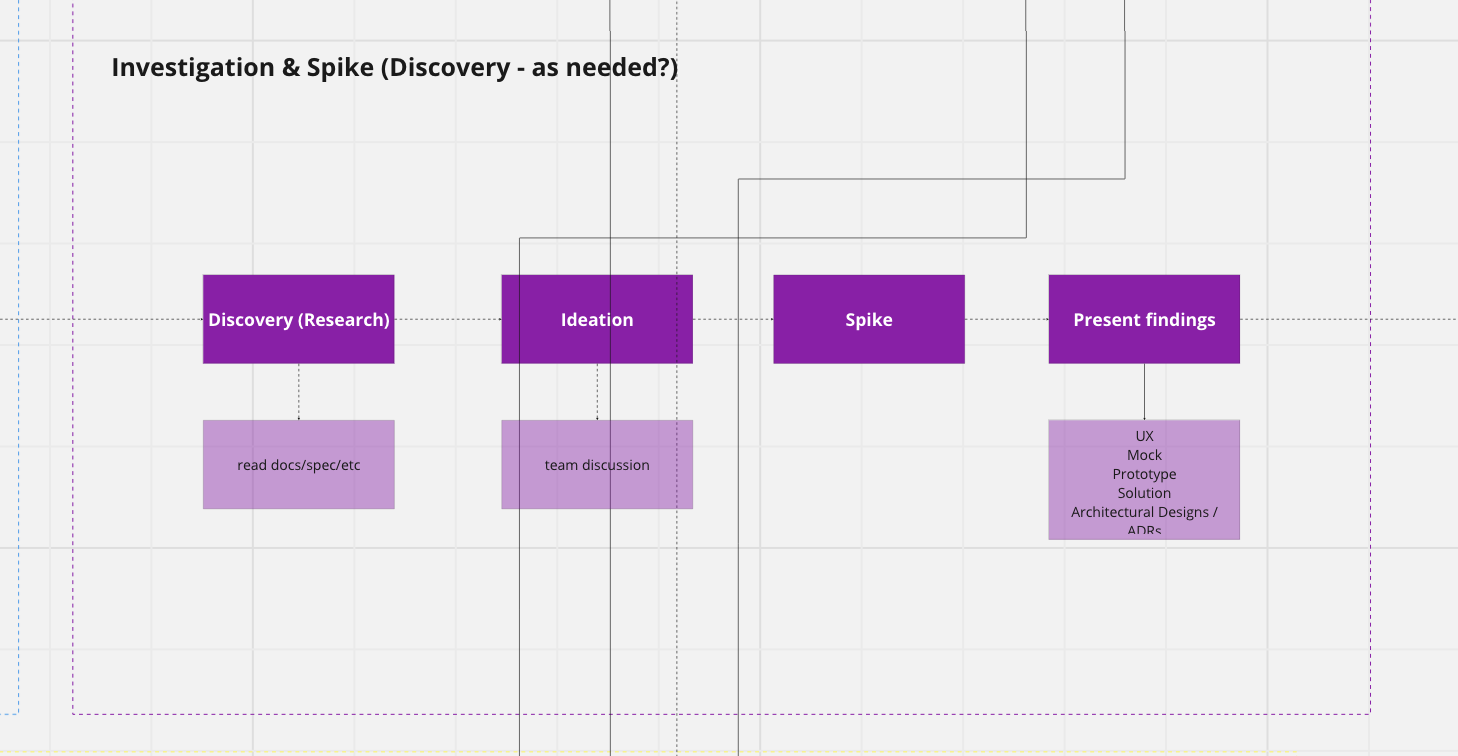
\includegraphics[width=8cm]{assets/workflow/investigation.png}
    \caption{Investigation stage of our ways of working.}
    \label{fig:workflowInvestigation}
  \end{figure}
  
  A spike is often used when there are unknowns about a  project (Visual Paradigm, 2024). A study done by 
  Hashimi and Gravell (2020) found that a majority of people in industry saw spikes as an effective tool and helped in managing risks. In another
  study they also stated that one of key purposes of a spike was to help guide story/ticket estimations (Hashimi, Gravell, 2019). 
  
  In the first paper it was also hypothesised that technical debt can also be lowered through the use of spikes, with technical debt be defined as:
  \begin{quote}
    \textit{'the idea that developers sometimes accept
    compromises in a system in one dimension (e.g., modularity) to meet an
    urgent demand in some other dimension (e.g., a deadline)' (Kruchten et al, 2012)}
  \end{quote}

  Spikes were used by Glas and Hedén (2021) to help bring down technical debt in their study. However when thought about simply, 
  a spike could be seen as a tool to spot the technical debt before it touches live systems. Due to a prototype being made flaws can be spotted 
  early and ironed out before the \textit{'real'} development work begins.

  For the project a spike was carried out to test the algorithms outlined in \hyperref[sec:AppendixC]{\textbf{Appendix C}} to test the 
  throughput of the system and see if it could handle the incoming requests. We used the technical spike template recommended by Microsoft (2021), to 
  document findings and outline the spikes objectives. Hashimi, Abduldaem and Gravell (2022) found that  \textit{'timeboxing, objectives,
  documentation, and clear communication'} were the key factors that lead to a successful spike.

  There was no time limit set, which did lead to scope creep (Martins, 2023) and more time being spent than was necessary. It's important to remember that a 
  spike is not meant to be the final product, however scope creep lead to the spike being almost a fully working system, albeit unrefined and with issues. 
  This is something as a team we have now changed in our process and will always timebox spikes in the future to prevent this.

  Despite this the other key factors were well adhered to. Objectives and documentation of the spike were put into a spike document
  and we had communication with a more senior member of the team at all times as well as daily stand ups to communicate issues/progress on the spike. 
  The full spike document can be seen in \hyperref[sec:AppendixE]{\textbf{Appendix E}}, below are the key findings.

  \begin{enumerate}
    \item A garbage collector should be used to clean up data that is no longer referenced by a schedule. This will help lower the amount of redis sets/gets
    and has no negative affect on partners.
    \item When a catalogue item (episode/series/brand) updates it will also need to update it's associated schedules, for titling and descriptions. This in 
    itself is not a problem, however if the number of schedules referenced is large it can significantly slow the system down. Parallelisation should be 
    looked into, at least at the schedule level to help ease this. Full parallelisation would require a new design to support parallelised editing of the 
    broadcast list held in episodes (this discussed in the \hyperref[sec:storageSolutions]{\textbf{Research}} section).
    \item Redis duplication is complex and is only needed so that episodes can reference a list of schedules that they are in. Might be worth using 
    DynamoDB here as this will also help with parallelisation (This is explored in the \hyperref[sec:future]{\textbf{Future Work}} section).
    \item Additional filtering from the catalogue pipeline could be added to only send updates for items that are referenced by a schedule. This would 
    stop lambda being ran that essentially do nothing, this is also discussed in \hyperref[sec:future]{\textbf{Future Work}}.
  \end{enumerate}

  It was determined by the team that, for now, the system should be single-threaded and stick to the original design due to time constraints.
  Parallelisation could be looked into in the future when we had some time. However it was agreed for a garbage collector to be used and 
  when a batch of schedule updates is is triggered by a catalogue update that some form of concurrency would be required. This can be done with schedule
  objects due to the single threaded nature of the current system. As the schedule updates are being done because of a catalogue update the only 
  fields that can change are the titles and descriptions. These do not affect or reference anything other than the object itself.

  \begin{figure}[H]
    \centering
    \includegraphics[width=8cm]{diagrams/activity/Schedule Concurrency.png}
    \caption{Simple activity diagram showing basic concurrency logic for updating schedules triggered by a catalogue update.}
    \label{fig:scheduleConcurrency}
  \end{figure}

  \newpage
  \subsection{Slicing and kick-off}
  Another small section is the \textit{'kick-off'}, usually a single meeting where the team gets together and discusses the tickets that makeup
  the project as a whole. 

  \begin{figure}[H]
    \centering
    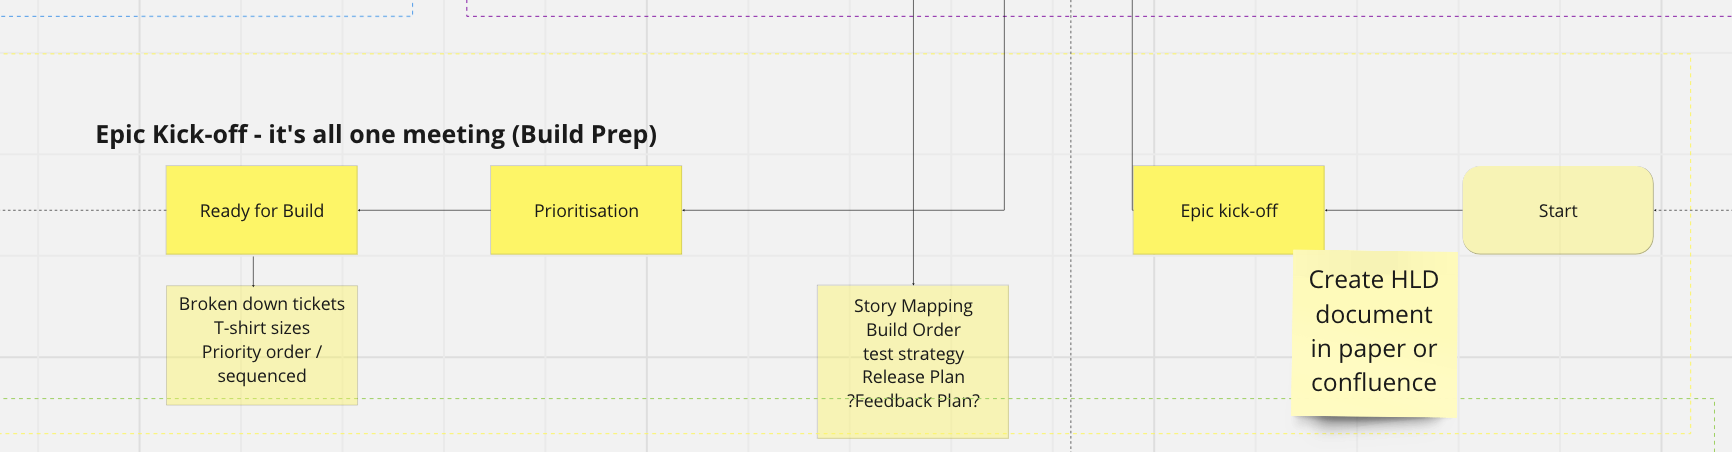
\includegraphics[width=8cm]{assets/workflow/kickoff.png}
    \caption{Kick-off stage of our ways of working.}
    \label{fig:workflowKickOff}
  \end{figure}
  
  Ideally this work has already been broken down into tasks. This is where the spike really helps, instead of guessing we are able to better understand 
  the work that needs doing and create tasks accordingly (Hashimi, Abduldaem, Gravell, 2022). The following diagram shows the initial breakdown of 
  tasks/tickets that were created for the project.

  \begin{figure}[H]
    \centering
    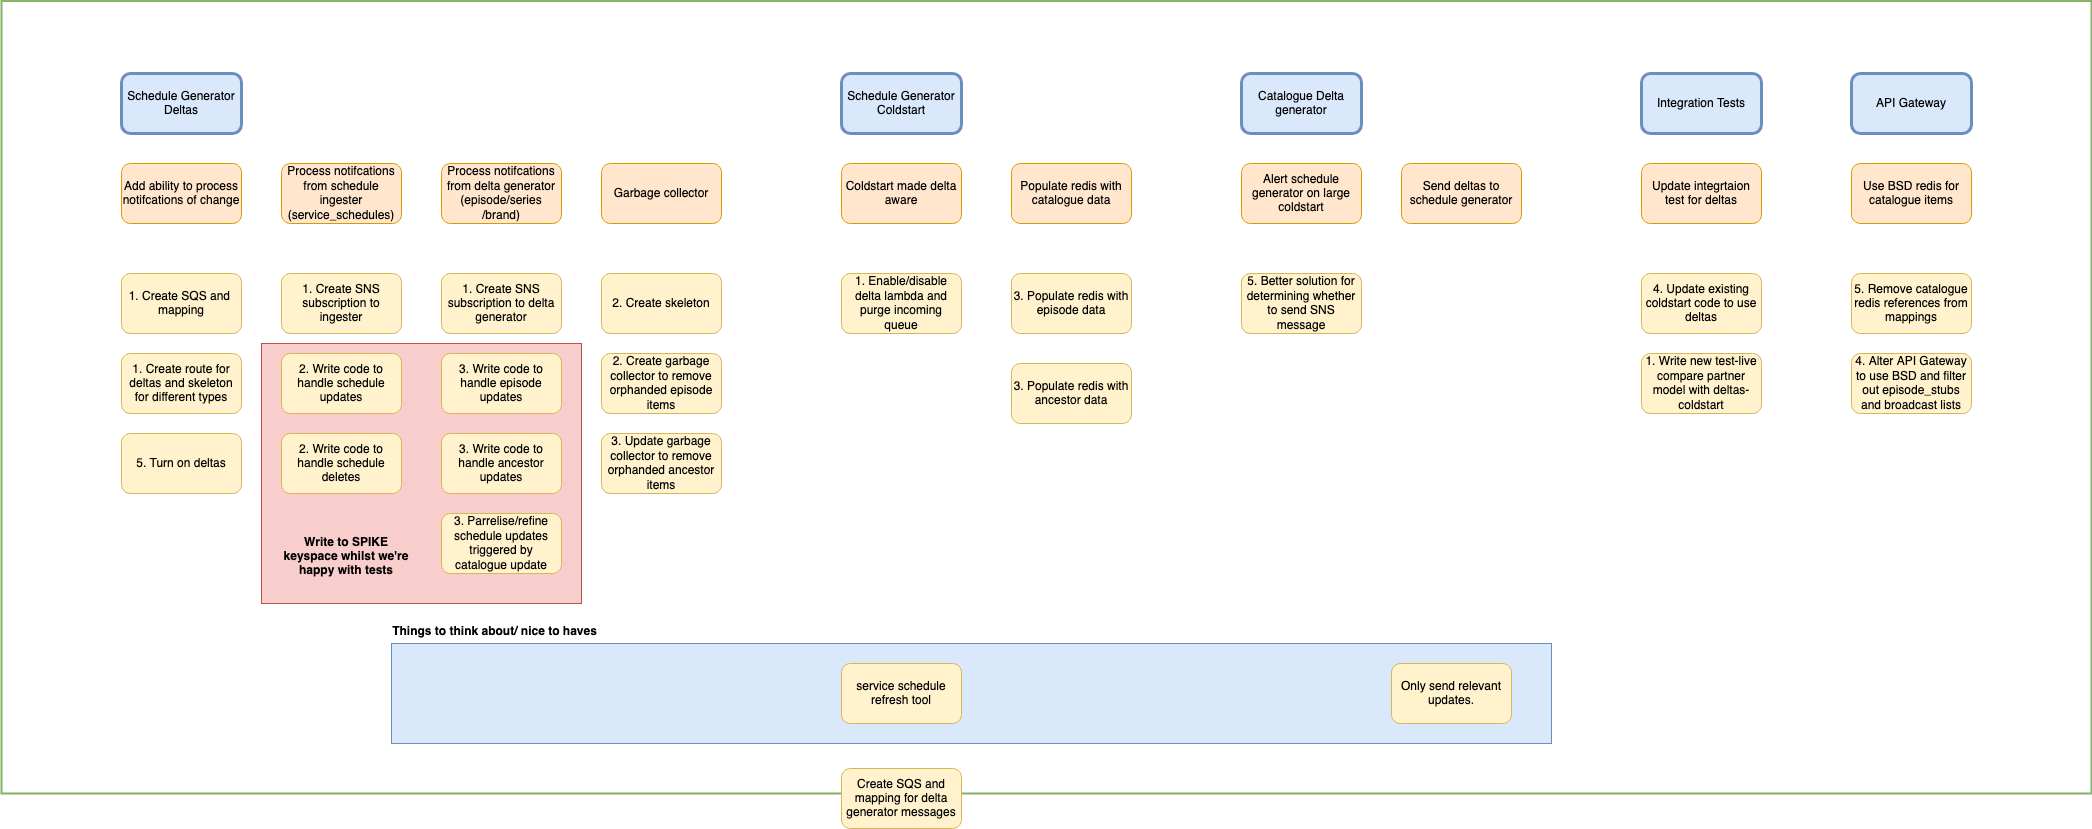
\includegraphics[width=14cm]{assets/schedulesSlicing.drawio.png}
    \caption{Pre-work slicing of work, organised vertically into components.}
    \label{fig:schedulesSlicing}
  \end{figure}

  A work breakdown structure (WBS) is a tool used to \textit{'break down deliverables into sub-deliverables to visualize projects'} (Raeburn, 2024) 
  and is typically broken down into 3 levels, parents, dependencies and sub-tasks, however it can consist of as any as a team wants. For the above I kept it 
  at 3 levels, going vertically, blue represents self-contained features/components, orange is a parent task to complete the feature and yellow is a 
  sub-task of the parent task. Numbers on the sub-tasks represent the initial prioritisation/ordering of the tasks into slices or feature sets.
  
  It's important to note that this is not the final list of tasks. Unknowns will always appear whilst developing the software and result in additional
  tasks being created. However the WBS helps refine the scope to what is needed (Burghate, 2018). As can be seen in the above figure there are 3 tasks that have 
  been moved to a \textit{'nice to have'} section, which have been deemed unnecessary for the projects initial completion.

  Another way to visualise these feature sets is using an Archimate implementation and migration diagram. This allows the modelling of work packages,
  gaps, deliverables, plateaus (stages) and events (The open group, 2016). The diagram on the next page shows the project mapped out using these elements, 
  documenting the deliverables for each feature set.

  \begin{figure}[H]
    \centering
    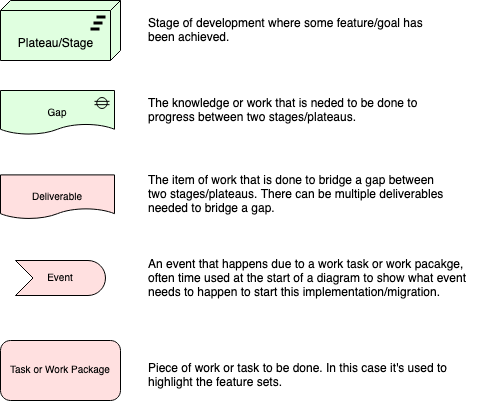
\includegraphics[width=6cm]{assets/migrationKey.drawio.png}
    \caption{Implementation and migration diagram components (The open group, 2016 and Jonkers et al, 2011).}
    \label{fig:migrationKey}
  \end{figure}

  \newpage

  \begin{landscape}
    \begin{figure}
      \centering
      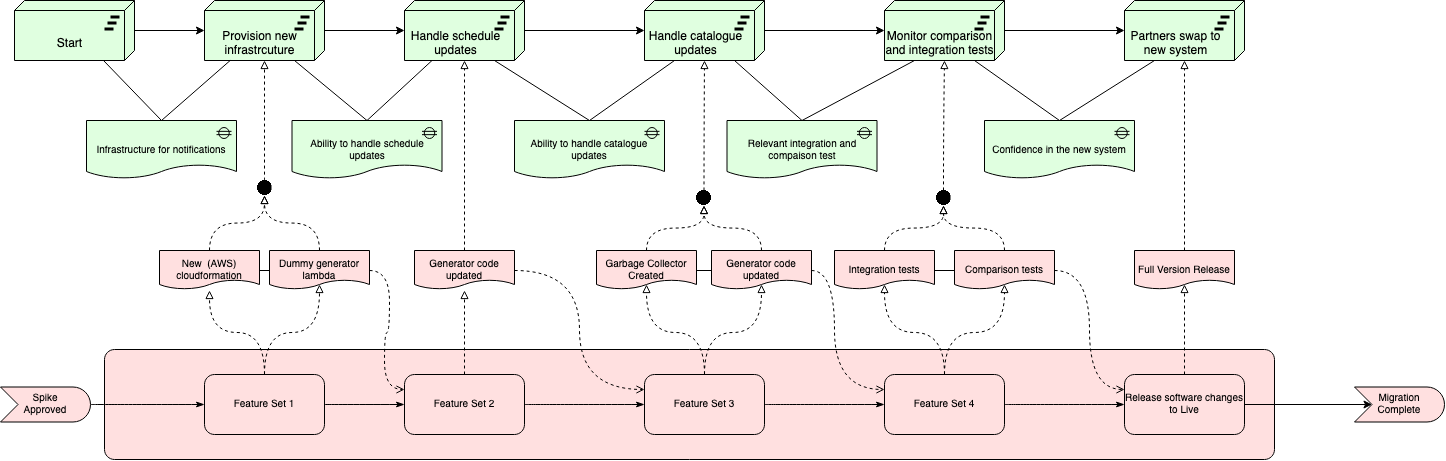
\includegraphics[width=20cm]{assets/migration.drawio.png}
      \caption{Figure showing Archimate implementation/migration diagram for project.}
      \label{fig:migration}
    \end{figure}
  \end{landscape}

  \newpage
  \subsection{Build software}
  Before discussing the build stage, it's important to understand the multiple environments used in development.

  \begin{figure}[H]
    \centering
    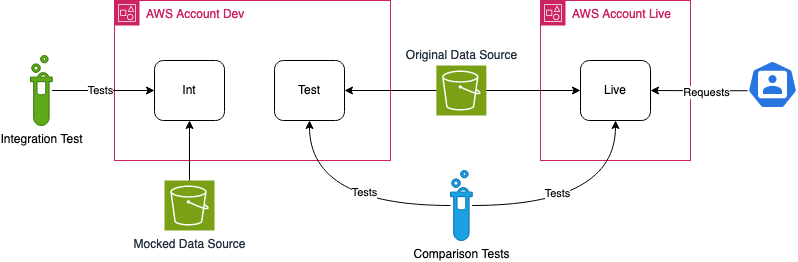
\includegraphics[width=8cm]{assets/environments.drawio.png}
    \caption{Diagram showing the different environments used by SpaceChimp.}
    \label{fig:environments}
  \end{figure}

  The above figure illustrates where the pipelines get their data from dependant on the environment, as well as what tests access said environment.
  We have 3 environments, int, test and live, with test mimicking live (Wiggins, 2017). This allows us to use the test environment to protect live from 
  any bugs or errors introduced by a task whilst also allowing the testing of outputs between old and software (Zheng, 2021). However when running on test
  and live we don't have control over the data source and the events it sends out to the pipeline, thus making it hard to test certain scenarios and features.
  This is where the int environment is used, we mock the data source used on test/live but have full control over what is added and removed, This allows 
  us to routinely check all edge cases and features are working as expected.

  \vspace{0.2cm}

  The build stage consists of writing and testing the software and resembles the flow of our kanban board.

  \begin{figure}[H]
    \centering
    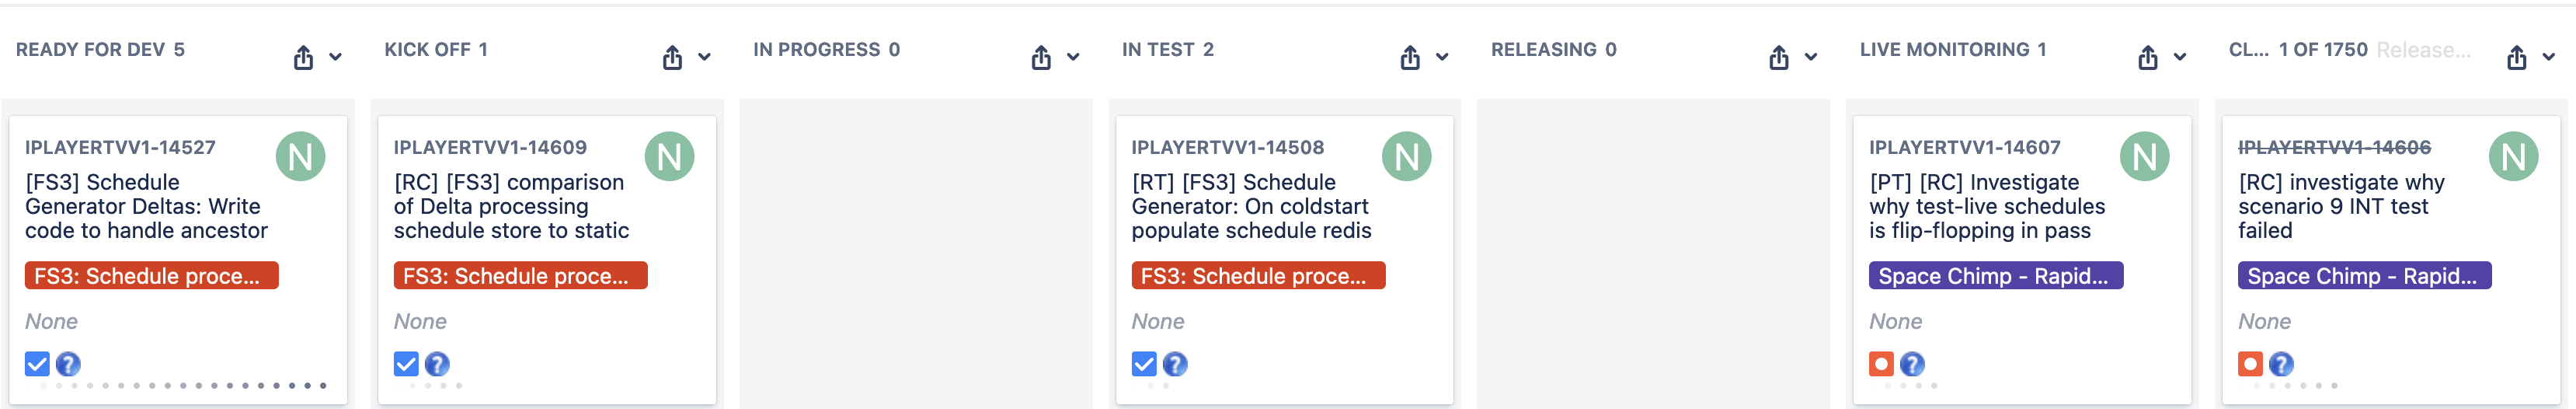
\includegraphics[width=10cm]{assets/kanbanBoard.png}
    \caption{SpaceChimps kanban board.}
    \label{fig:kanbanBoard2}
  \end{figure}

  \begin{itemize}
    \item \textbf{Ready for dev} - Tasks that are ready to be picked up for development.
    \item \textbf{Kick-off} - Tasks that need a test kick-off, which is not the same as the previous sections kick-off. This is where developers
    discuss the task with a member of the test team and determine the Acceptance Criteria (ACs) and test approach for the task.
    \item \textbf{In Progress} - Tasks that are being developed and worked on.
    \item \textbf{In Test} - Task has been completed and changes are on the test environment. A member of the test team can now test the ticket
    based on the previous discussions had in the kick-off. If things have changed during development, an additional hand-over with the test team 
    is done to discuss the new changes.
    \item \textbf{Releasing} - After a ticket task has been tested and has met the specified ACs, the task is moved to the releasing column signifying 
    that is ready to be deployed to the live environment.
    \item \textbf{Live monitoring} - Tasks in this column need to be monitored on the live environment to make sure that the change is functioning as expected.
  \end{itemize}

  \begin{figure}[H]
    \centering
    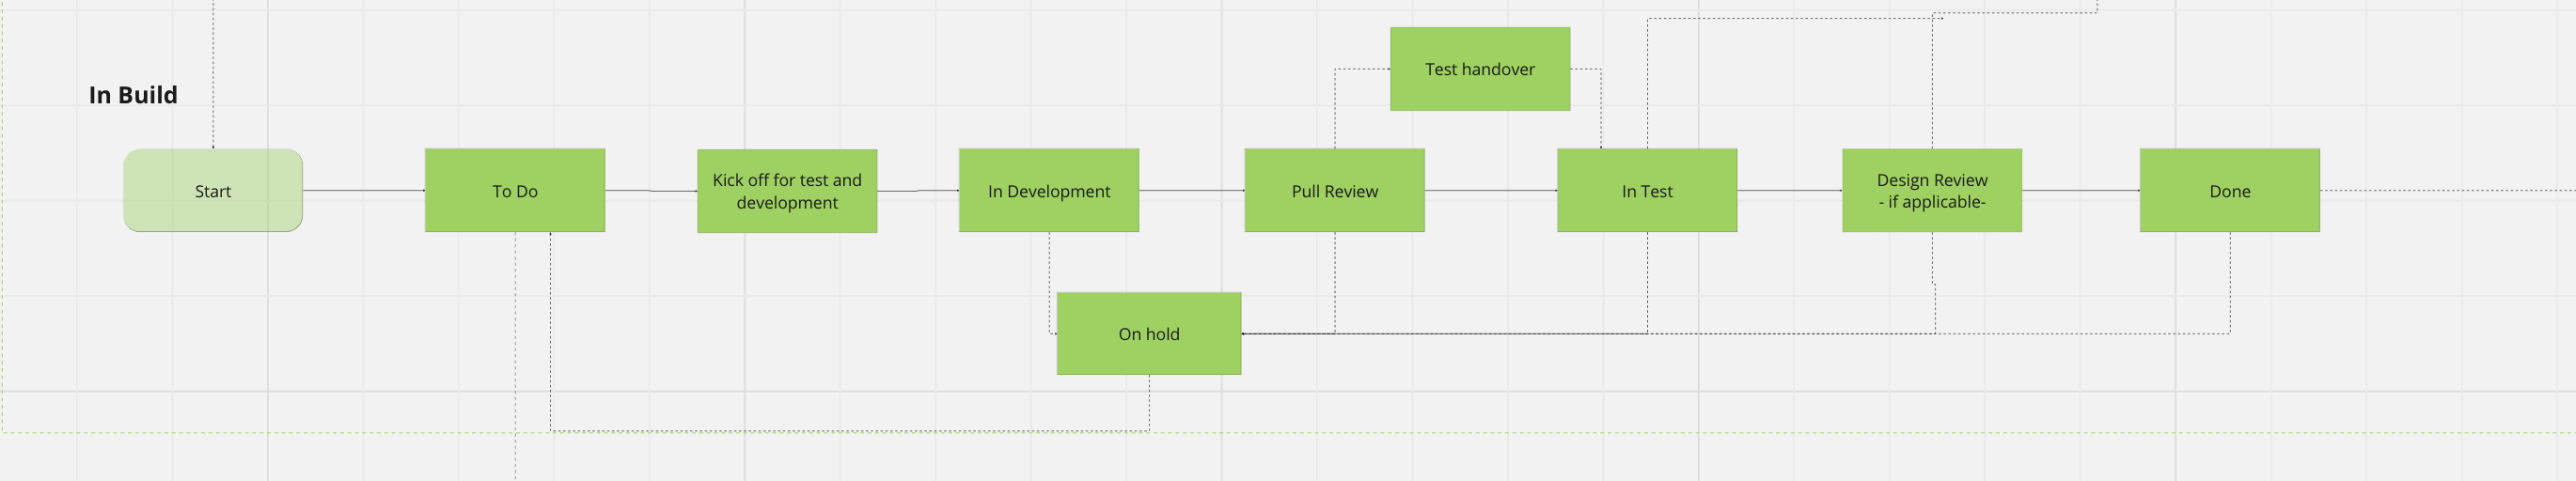
\includegraphics[width=8cm]{assets/workflow/build.png}
    \caption{Build stage of our of working.}
    \label{fig:workflowBuild}
  \end{figure}

  I will now discuss the 4 key components/features that were built during this stage, along with decisions and challenges that occurred during development.

  \subsubsection{Coldstarts}

  \subsubsection{Delta/change lambda}

  \subsubsection{Garbage Collector}

  \subsubsection{Integration tests}

  \newpage
  \subsection{Release}
  The release stage is the final stage in our workflow. This is when software gets released to the live environment and becomes available to partners. 
  \begin{figure}[H]
    \centering
    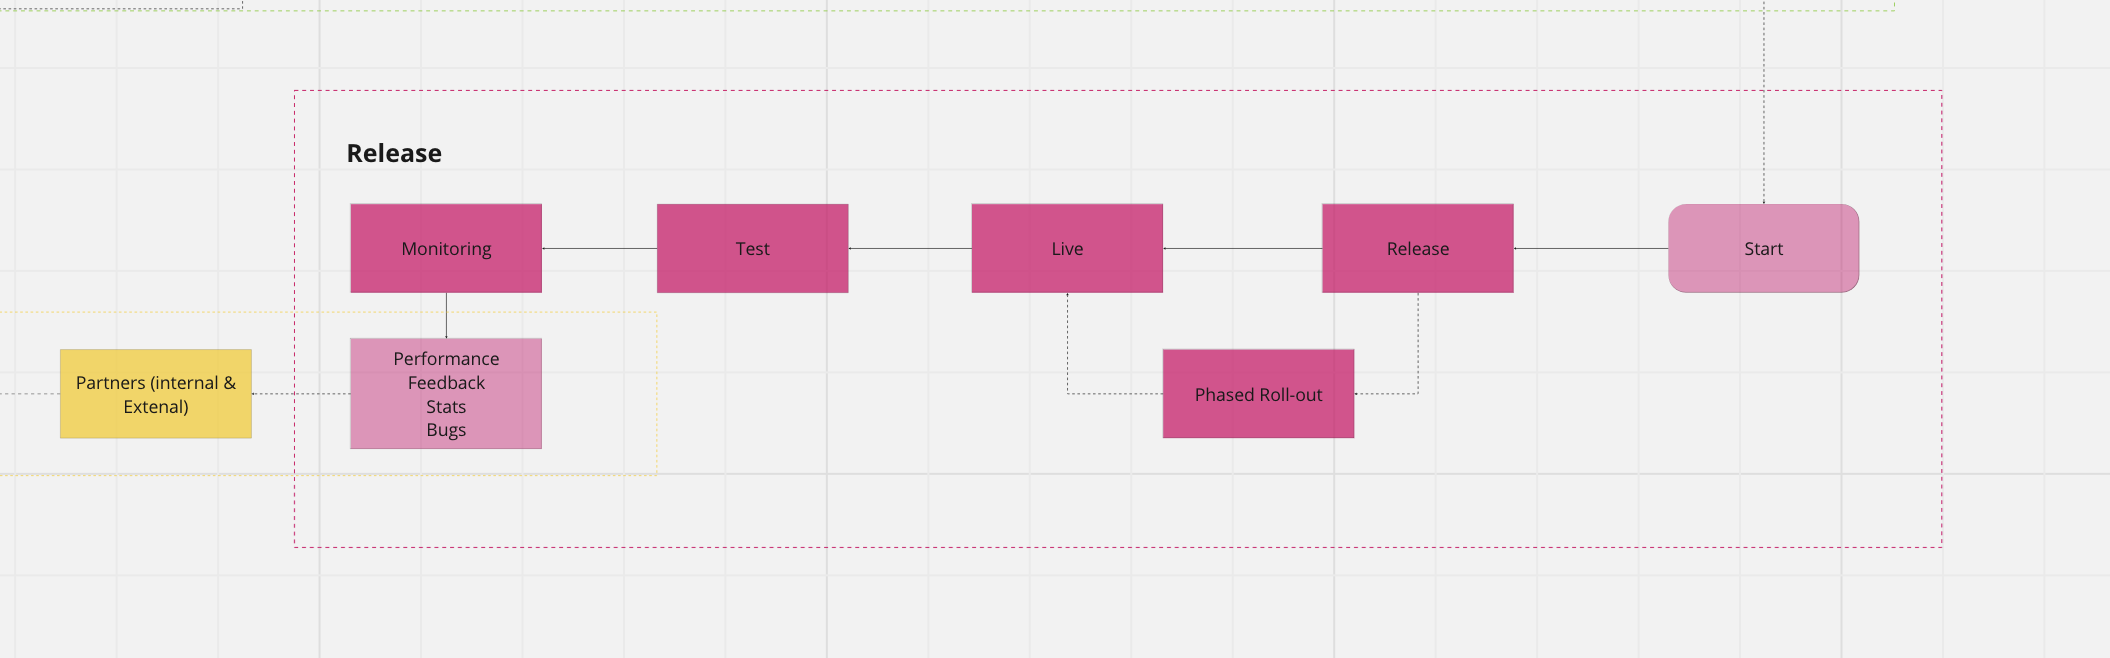
\includegraphics[width=8cm]{assets/workflow/release.png}
    \caption{Release stage of our ways of working.}
    \label{fig:workflowRelease}
  \end{figure}
  
  However in this case it doesn't become available to partners until we have confidence in the new system. We have config for each partner that 
  specifies what data they have access to. In the case of schedules, this includes keyspace information on where the data is retrieved from. As 
  previously discussed in the \hyperref[sec:cicd]{\textbf{Research}} section, the new and old system will run in parallel until our comparison tests 
  convince us that the new system outputs the same as the old.

  \begin{figure}[H]
    \centering
    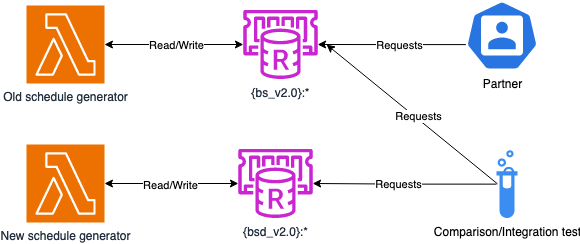
\includegraphics[width=8cm]{assets/keyspaceAccess.drawio.png}
    \caption{Diagram showing access to keyspaces.}
    \label{fig:keySpaceAccess}
  \end{figure}

  Until then partners will still access data from the old system, with a simple config change being the rollover/rollback mechanism. If we wanted we 
  could setup an automatic rollback and huddle system (Sathre, Zambreno, 2008), with the huddle portion consisting of developers being called out if 
  outside of working hours to monitor and remedy the situation. This can be done in many ways but one way would be through AWS alarm 
  actions (Amazon Web Services, 2024k). An alarm going into error would  triggers a rollback of the configs version in S3 (Amazon Web Services, 2024d).

  \begin{figure}[H]
    \centering
    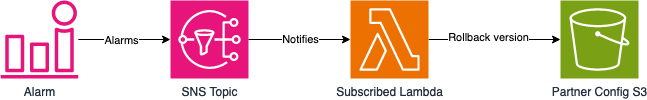
\includegraphics[width=8cm]{assets/rollback.drawio.png}
    \caption{Automatic rollback architecture on alarm error.}
    \label{fig:rollback}
  \end{figure}

  For our case this is most likely over-engineering and unnecessary. A config change only takes a minute to do and if there ever was an error we 
  would be notified and called out to fix the problem when necessary. 

  Once the switchover happens we wait for partner feedback and use created dashboards, these will be shown in the next section, to monitor 
  the new software. Alongside this, our comparison test and side-by-side running of new and old systems will continue for a short while after release, 
  allowing an easy rollback to the old system. Next this old lambdas scheduler will be disabled, but the lambda itself kept in case of an emergency. 
  Finally, after sufficient time has passed the old system can be deconstructed and removed completely.

\newpage
